\chapter{Где учатся и кем работают изобретатели языков программирования}
\label{ch:programming languages}

В статье исследуются свойства языков программирования на основе базы знаний международного проекта Викиданные. С помощью SPARQL-запросов, вычисляемых на объектах типа "язык программирования" в Викиданных, решен ряд задач. Получены перечени всех языков программирования под пермиссивными лицензиями и языков с закрытыми лицензиями и рассчитано их процентное соотношение. Построена пузырьковая диаграмма по количеству форматов файлов исходного кода. Получены карты, отображающие месторасположение учебных заведений и компаний, в которых учились или работали люди, связанные с созданием языков программирования. Построена пузырьковая диаграмма, отображающая профессии людей, причастных к созданию и разработке языков программирования. Получен список всех объектно-ориентированных языков программирования и сделан вывод об исчерпывающей полноте Викиданных относительно них. Проведено сравнение и анализ результатов SPARQL-запросов 2017 года и 2020 года, отмечены основные изменения. 

%%
% Постановка задачи
%%
\section{Постановка задачи}
Исследуем языки программирования, а именно информацию о них в Русской Википедии, Английской Википедии и Викиданных.
Задачи:
\begin{enumerate} 
  \itemПостроить упорядоченный список языков программирования по числу интервик.
  \itemПостроить список языков по числу посещений статей в Русской Википедии.
  \itemПостроить направленный ациклический граф зависимостей языков программирования друг от друга (или найти циклы в зависимостях, если такой граф нельзя построить). См. свойство "influenced by"\  в Java.
\end{enumerate}

\textbf{Экземпляры объекта "Язык программирования"}
\begin{itemize}
\itemОбъекты: язык программирования (Q9143).
\itemСвойства: instance of (P31).
\end{itemize}

\begin{lstlisting}[
	language=SPARQL,
	label=lst:prog_langs,
	caption={\href{https://w.wiki/kCe}{Список языков программирования}\protect\footnotemark},
	texcl 
]
#added 2016-10
#List of `instances of` "programming language" 
SELECT ?lang ?langLabel
WHERE
{
    ?lang wdt:P31 wd:Q9143. # instances of programming language
    SERVICE wikibase:label { bd:serviceParam wikibase:language "ru"}
}
\end{lstlisting}
\footnotetext{Результатом запроса~\ref{lst:prog_langs} является список всех языков прогрмаммирования. На 2017 год список содержал 732 записи, а на 2020 год число языков программирования увеличилось до \num{1422} записи.}


Наиболее полными и проработанными языками программирования на Викиданных на 2017 год являются: Java, Python, C. На 2020 год наиболее проработанными на Викиданных языками программирования являются: C++ (26 свойств), Java (26 свойств), JavaScript (25 свойств), R (25 свойств).
Почти пустыми и малоинформативными языками на 2017 год оказались: CLIPS, Dylan, Go!.
Недостаток полученного списка в том, что ряд объектов получился безымянным на Викиданных (No label defined). Попробуем получить список языков, у которых поле "label"\  будет непустым.

\begin{lstlisting}[
	language=SPARQL,
	label=lst:labeled_languages,
	caption={\href{https://w.wiki/kCf}{Список языков программирования с заполненным свойством label}\protect\footnotemark},
	texcl
]
#List of `instances of` "programming language"\  only with a label.
SELECT ?item ?item_label
WHERE
{
    ?item wdt:P31 wd:Q9143 # instances of programming language
    ; rdfs:label ?item_label . 

    FILTER (LANG(?item_label) = "ru") . 
}
\end{lstlisting}
\footnotetext{Результатом запроса~\ref{lst:labeled_languages} также будет список языков программирования, но из неё исключены те, для которых не указан параметр label. На 2017 год список содержит 709 записей, на 2020 год в списке 1422 записи. Если в 2017 году на два десятка записей стало меньше, то в 2020 год все языки в списке имеют заполненное поле label.}

%%
% Демонстрация работы с операциями над множества в SPARQL
%%
Вывести все языки программирования, являющиеся открытым программным обеспечением (free software) и/или испытавшие на себе влияние, хотя бы одного из следующих языков программирования: Си, Python, Java. При этом разработанные какой-либо из фирм, кроме: Sun Microsystems, Космический центр имени Линдона Джонсона.

Используются:
\begin{itemize}
\itemОбъект: programming language (Q9143).
\itemСвойство: influenced by (P737).
\itemСвойство: developer (P178).
\end{itemize}

\begin{lstlisting}[
	language=SPARQL,
	label=lst:free_license_languages,
	caption={\href{https://w.wiki/kCh}{Пример более сложного SPARQL-запроса}\protect\footnotemark},
	texcl
]
#2017-02
SELECT DISTINCT ?item ?item_label
WHERE
{
    ?item wdt:P31 wd:Q9143 # instances of programming language
    ; rdfs:label ?item_label . 

    FILTER (LANG(?item_label) = "ru") . 

    {
      { ?item wdt:P737 wd:Q15777 } UNION # influenced by C
      { ?item wdt:P737 wd:Q28865 } UNION # influenced by Python
      { ?item wdt:P737 wd:Q251   } UNION # influenced by Java
      { ?item wdt:P31  wd:Q341   }
    } MINUS 
  	{ 
      { ?item wdt:P178 wd:Q14647  } UNION # developer Sun Microsystems
      { ?item wdt:P178 wd:Q208371 }       # developer Lyndon Johnson
    }  										    # Space Center
}
\end{lstlisting}
\footnotetext{Рeзультатом запроса~\ref{lst:free_license_languages} является список языков программирования, удовлетворяющих указанным выше требованиям. На 2017 год список содержил 115 записей, на 2020 год - 112 записей.}


%%
% Пермессивные лицензии
%%
Выведем все языки программирования находящиеся под пермиссивными лицензиями (практически не ограничивают свободу действий пользователей ПО и разработчиков).

Используются:
\begin{itemize}
\itemОбъект: programming language (Q9143).
\itemСвойство: license (P275).
\end{itemize}

\begin{lstlisting}[
	language=SPARQL,
	label=lst:permessive_license,
	caption={\href{https://w.wiki/kD6}{Языки программирования с пермессивными лицензиями}\protect\footnotemark},
	texcl
]
SELECT DISTINCT ?item ?item_label
WHERE
{
    ?item wdt:P31 wd:Q9143 # instances of programming language
    ; rdfs:label ?item_label . 

    FILTER (LANG(?item_label) = "ru") . 
  
      { ?item wdt:P275 wd:Q308915  }  UNION  # license Mozzila Public
      { ?item wdt:P275 wd:Q334661  }  UNION  # license MIT
      { ?item wdt:P275 wd:Q191307  }  UNION  # license BSD
      { ?item wdt:P275 wd:Q6905323 }         # license CC
}
\end{lstlisting}
\footnotetext{Результатом работы запроса~\ref{lst:permessive_license} является список языков программирования, находящихся под пермиссивными лицензиями. На 2017 год список содержал 37 записей, на 2020 год в списке 82 записи. В этот список из 82 "свободных"\  языков попали, например CoffeeScript, Go, Haml.}

Рассмотрим соотношение языков с пермиссивной лицензией и языков с проприетарной или закрытыми лицензиями.
\begin{lstlisting}[
	language=SPARQL,
	label=lst:license_compare,
	caption={\href{https://w.wiki/kD6}{Рассчёт отношения "свободных"\ языков к "закрытым".}\protect\footnotemark},
	texcl
]
#2020-10-07
#The script calculates the percentage of programming languages 
#with a free license in relation to languages with a closed license
SELECT (COUNT(?not_free)* 100 / (COUNT(?free)) as ?total) WHERE
{ 
{
    SELECT ?free WHERE 
    {
         ?free wdt:P31 wd:Q9143 # instances of programming language
         ; rdfs:label ?item_label . 

         FILTER (LANG(?item_label) = "ru") . 
  
         { ?free wdt:P275 wd:Q308915  }  UNION  # license Mozzila Public
         { ?free wdt:P275 wd:Q334661  }  UNION  # license MIT
         { ?free wdt:P275 wd:Q191307  }  UNION  # license BSD
         { ?free wdt:P275 wd:Q6905323 }         # license CC
    }
}
UNION
{
    SELECT ?not_free WHERE 
    {
      ?not_free wdt:P31 wd:Q9143 # instances of programming language
      ; rdfs:label ?lang_label . 
      FILTER (LANG(?lang_label) = "ru") .
  
      { ?not_free wdt:P275 wd:Q6165015 } UNION # Java Research License
      { ?not_free wdt:P275 wd:Q218616 } UNION # proprietary software
      { ?not_free wdt:P275 wd:Q3238057 } UNION # proprietary license 
      { ?not_free wdt:P275 wd:Q31202214 } UNION # proprietary software 
      { ?not_free wdt:P275 wd:Q979794 } # Aladdin Free Public License
    }
}
}
\end{lstlisting}
\footnotetext{Рeзультатом запроса~\ref{lst:license_compare} будет значение отношения числа языков программирования со свободной лицензией к числу языков с закрытой лицензией. На 2020 год это значение равно 20\%.}

%%
% Количество форматов файлов исходного кода
%%
\section{Количество форматов файлов исходного кода}
В зависимости от языка программирования, файлы с исходным кодом программ могут иметь разные расширения. Построим пузырьковую диаграмму по количеству допустимых форматов файлов исходного кода и сравним с аналогичной диаграммой, построенноый в 2017 году.

На рисунке рис. ~\ref{fig:source_file_formats_2017} видно, что на 2017 год самыми исторически богатыми на форматы и расширения файлов являлись такие языки программирования, как: C++ (10 форматов), Geometric Description Language (8), Racket (7). Причем стоит заметить, что соотношение один язык программирования - один формат файлов исходного кода не является верниы. Например, файлы с программой на языке Racket могут иметь расширения rkt, rktl, rktd, scrbl, plt, ss или scm.

\begin{figure}[h]
\centering
	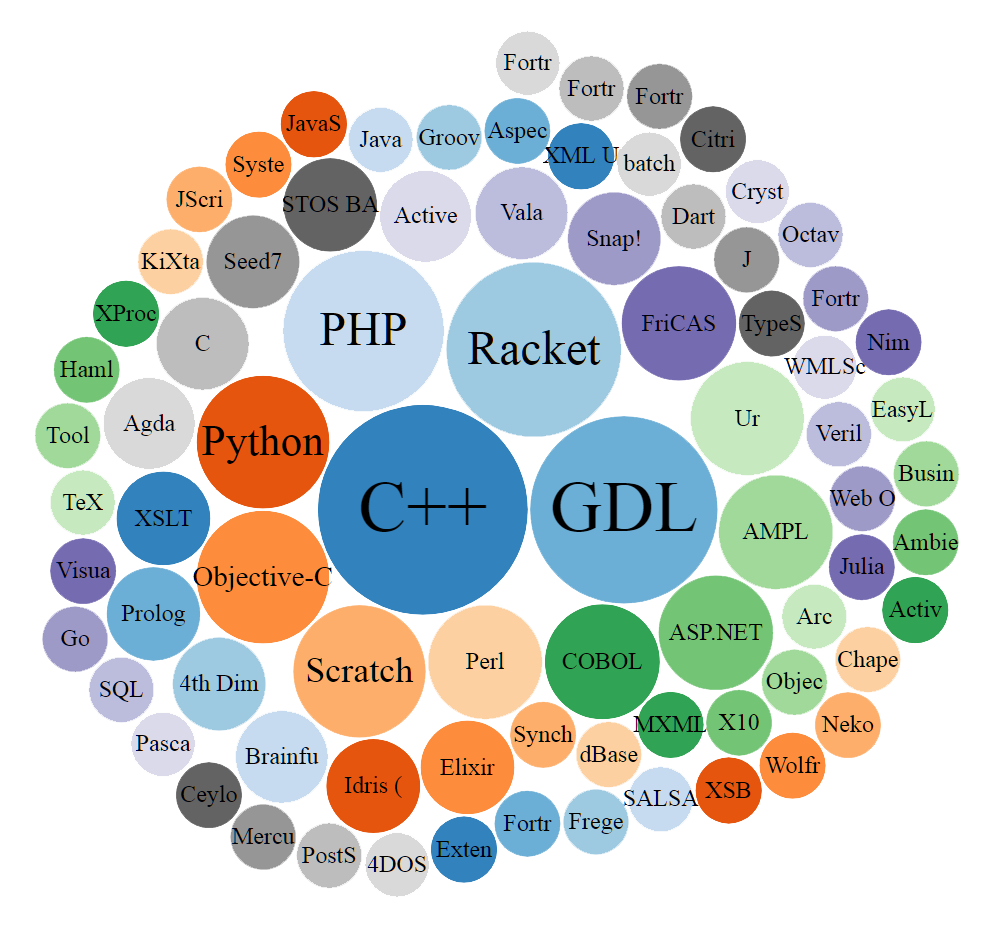
\includegraphics[width=0.7\textwidth]{./chapter/programming_language/File_extensions_quantity_of_source_code_2017.png}
	\caption{Пузырьковая диаграмма по количеству форматов файлов исходного кода на 2017 год.}
	\label{fig:source_file_formats_2017}
\end{figure}

К 2020 году (рис. ~\ref{fig:source_file_formats_2020}) C++ и Geometric Description Language (GDL) остались на лидирующем месте (10 и 8 форматов-расширений). За три года подтянулись и вошли в первую восьмёрку также такие языки, как Raku (9 форматов), REXX и Scratch (по 6 форматов), Java и Wolfram Language (по 5 форматов).

\begin{figure}[h]
\centering
	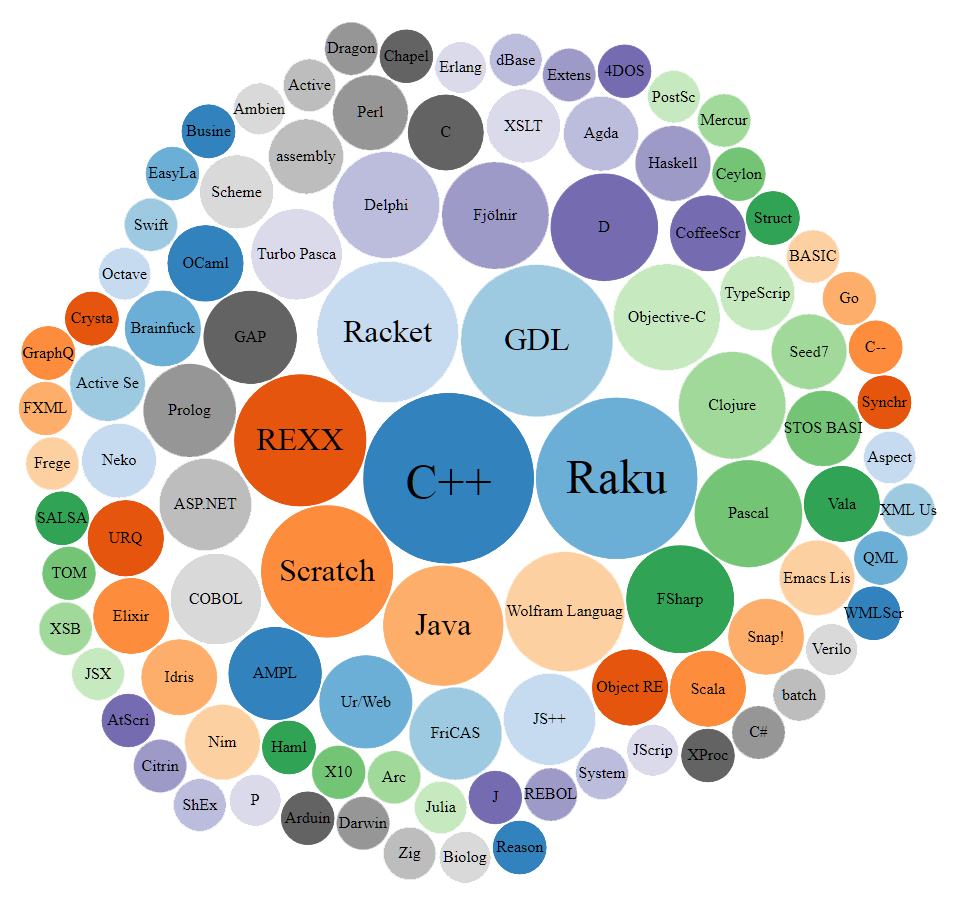
\includegraphics[width=0.7\textwidth]{./chapter/programming_language/File_extensions_quantity_of_source_code_2020.png}
	\caption{Пузырьковая диаграмма по количеству форматов файлов исходного кода на 2020 год.}
	\label{fig:source_file_formats_2020}
\end{figure}

Из этого можно сделать вывод, что развитие языков программирвоание продолжается непрерывно, постоянно возникают новые форматы файлов исходного кода, но лидеры в этой области не спешат сдавать свои позиции.

%%
% Страны, в которых живут люди и располагаются организации, связанные с созданием языков программирования
%%
\section{Страны, в которых живут люди и располагаются организации, связанные с созданием языков программирования}

Отобразим на карте страны, в которых живут люди и располагаются организации, связанные с созданием языков программирования. Заметим, что разработчиком языка может выступать как организация, так и отдельных человек. Для определения месторасположения (свойство: coordinate location) организации будем использовать координаты её штаб-квартиры (свойство: headquarters location), для человека - координаты места его рождения (свойство: place of birth).

Используются:
\begin{itemize}
\itemОбъект: programming language (Q9143).
\itemСвойство: instance of (P31).
\itemСвойство: developer (P178).
\itemСвойство: headquarters location (P159).
\itemСвойство: place of birth (P19).
\itemСвойство: coordinate location (P625).
\end{itemize}

\footnotetext{Результатом запроса ~\ref{lst:countries_map} является карта, где красными точками указаны места проживания людей, причастных к разработке языков программирования. На рисунке рис. ~\ref{fig:countries_2017} изображен результат запроса на 2017 год, а на рис. ~\ref{fig:countries_2020} показаны аналогичные данные на 2020 год.}
\begin{lstlisting}[
	language=SPARQL,
	label=lst:countries_map,
	caption={\href{https://w.wiki/kD9}{Карта с указанием места жительства или работы разработчиков языков программирования}\protect\footnotemark},
	texcl
]
#2017-05
#defaultView:Map
SELECT ?item_label ?developer_label ?location_label ?coord
WHERE
{
    ?item wdt:P31 wd:Q9143 # instances of programming language
    ; rdfs:label ?item_label.     
    FILTER (LANG(?item_label) = "ru"). 
  
    ?item wdt:P178 ?developer. # developer
    ?developer rdfs:label ?developer_label. 
    FILTER (LANG(?developer_label) = "ru"). 
      		
    { ?developer wdt:P159 ?location. } UNION # headquarters location
    { ?developer wdt:P19  ?location  }       # place of birth
    ?location rdfs:label ?location_label. 
    FILTER (LANG(?location_label) = "ru").
    
    ?location wdt:P625 ?coord. # coordinate location

    SERVICE wikibase:label {
        bd:serviceParam wikibase:language "ru".
    }   	
}
\end{lstlisting}

\begin{figure}[h]
\centering
	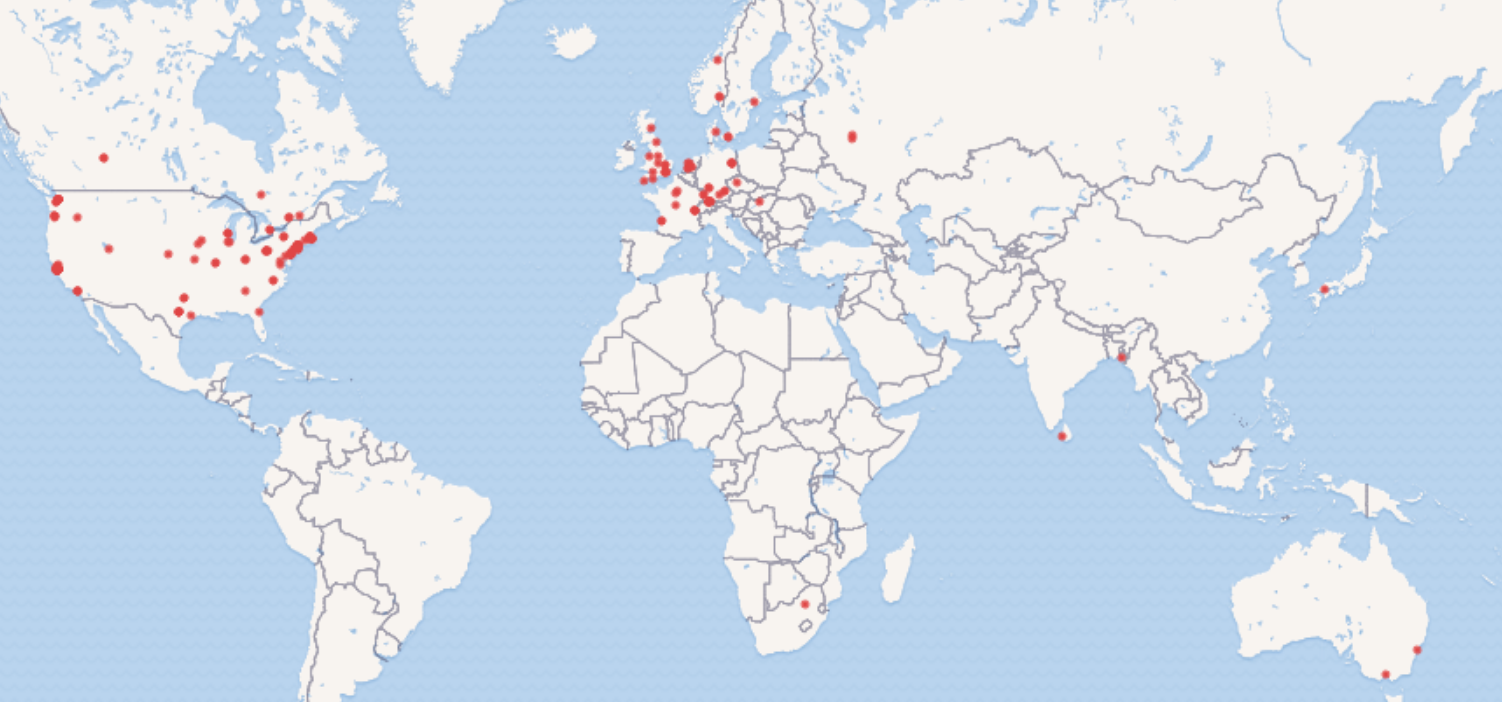
\includegraphics[width=1\textwidth]{./chapter/programming_language/Map_showing_contries_2017.png}
	\caption{Страны, в которых живут люди и организации, связанные с созданием языков программирования (2017).}
	\label{fig:countries_2017}
\end{figure}
\begin{figure}
\centering
	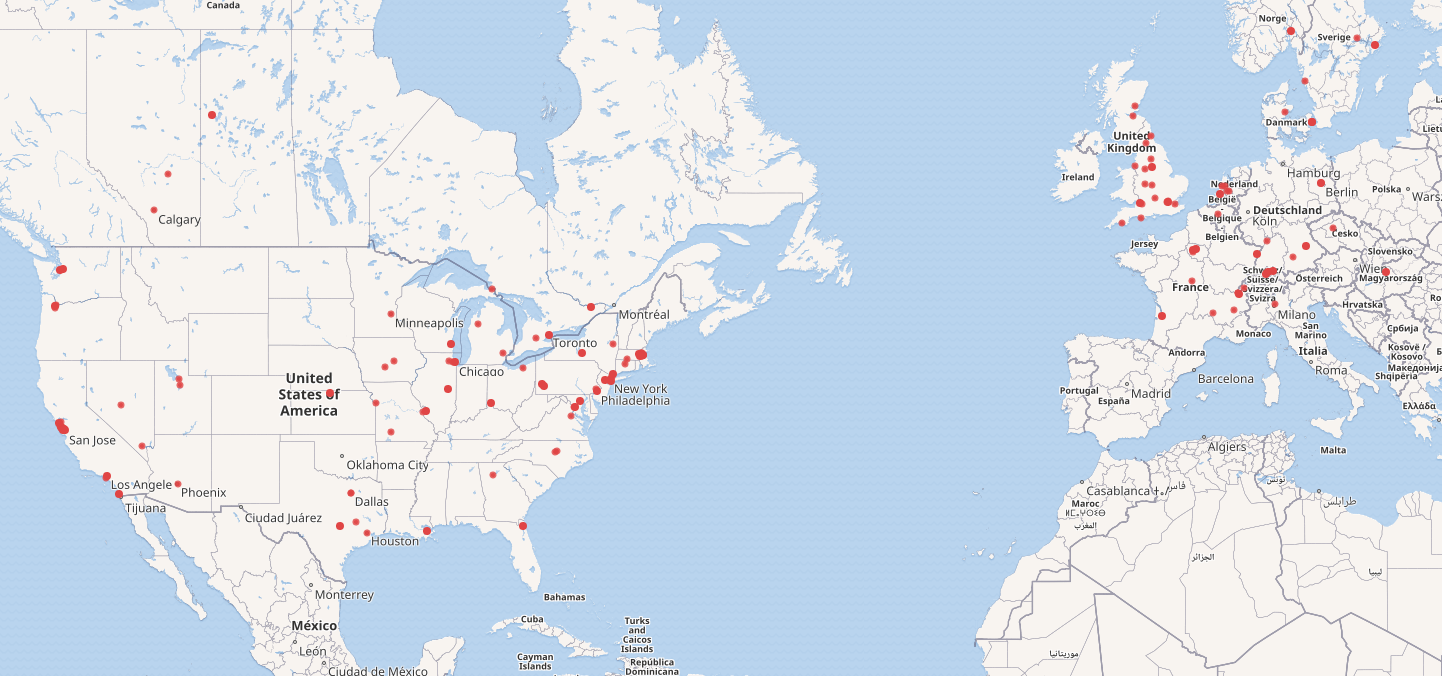
\includegraphics[width=1\textwidth]{./chapter/programming_language/Map_showing_contries_2020.png}
	\caption{Страны, в которых живут люди и организации, связанные с созданием языков программирования (2020).}
	\label{fig:countries_2020}
\end{figure}

\begin{marginfigure}
{
\setlength{\fboxsep}{0pt}%
\setlength{\fboxrule}{1pt}%
\fcolorbox{white}{white}{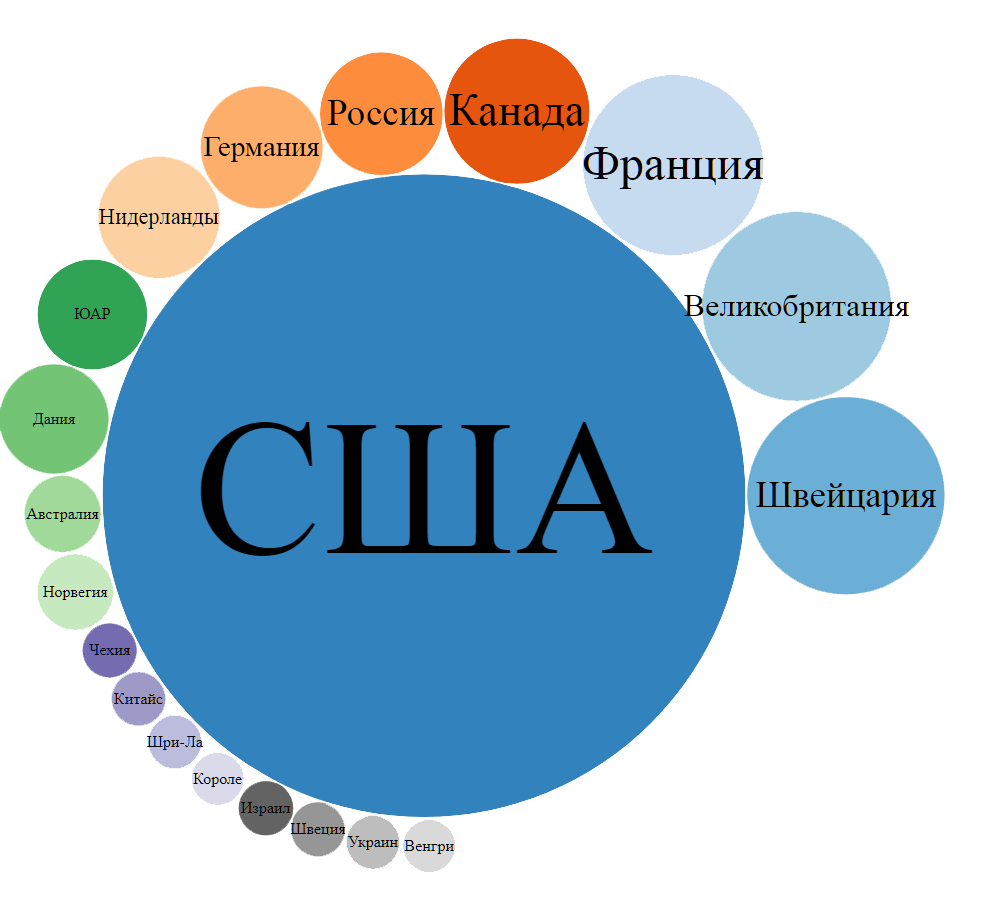
\includegraphics[width=\linewidth]{./chapter/programming_language/The_most_favorable_countries_for_the_emergence_of_people_capable_of_developing_programming_languages_2020_RU.png}}%
}
  \caption{Наиболее благоприятные страны для появления людей, способных к разработке языков программирования на 2020 год.}%
  \label{fig:countries_2_2020}%
\end{marginfigure}
По  рис. ~\ref{fig:countries_2017} и рис. ~\ref{fig:countries_2020} можно сделать вывод, что наиболее благоприятными местами жительства для людей, разрабатывающих языки программирования являются восточное побережье США, центральная европа и Великобритания.

Построим также пузырьковую диаграмму, чтобы выявить наиболее благоприятные страны для появления людей, способных к разработке языков программирования и размещению в этих странах штаб-квартир. Видим на рисунке, что наиболее благоприятными странами оказались США (159 человек и штаб квартир) и Великобритания (15). В России было разработано только два языка программирования: РЕФАЛ и Встроенный язык программирования 1С:Предприятие.

На 2020 год (рис. ~\ref{fig:countries_2_2020}) число штаб-квартир в США равно 241, в Великобритании — 24, в Франции — 18, а в России — 5.

%%
% Университеты, в которых учились люди, разрабатывавшие языки программирования
%%
\section{Университеты, в которых учились люди, разрабатывавшие языки программирования}
Отобразим на карте учебные заведения, в которых учились студенты, впоследствии разработавшие языки программирования.

Используются:
\begin{itemize}
\itemОбъект: programming language (Q9143).
\itemСвойство: instance of (P31).
\itemСвойство: developer (P178).
\itemСвойство: educated at (P69).
\itemСвойство: coordinate location (P625).
\end{itemize}


\footnotetext{Результатом запроса~\ref{lst:developer_university} будет карта, на которой красными точками отмечены места расположения университетов, в которых учились люди, создавшие языки программирования. На 2017 год получено 142 записи, к 2020 число записей увеличилось до 282.}
\begin{lstlisting}[
	language=SPARQL,
	label=lst:developer_university,
	caption={\href{https://w.wiki/kDY}{Карта с указанием университетов, в которых учились разработчики языков программирования}\protect\footnotemark},
	texcl
]
#2017-05
#defaultView:Map
SELECT ?item_label ?developer_label ?educational_institution_label ?coord
WHERE
{
    ?item wdt:P31 wd:Q9143 # instances of programming language
    ; rdfs:label ?item_label. 
    FILTER (LANG(?item_label) = "ru"). 
    
    ?item wdt:P178 ?developer. # developer
    ?developer rdfs:label ?developer_label. 
    FILTER (LANG(?developer_label) = "ru"). 
    	
    ?developer wdt:P69 ?educational_institution. # educated at
    ?educational_institution rdfs:label ?educational_institution_label. 
    FILTER (LANG(?educational_institution_label) = "ru").
    
    ?educational_institution wdt:P625 ?coord. # coordinate location
    
    SERVICE wikibase:label {
        bd:serviceParam wikibase:language "ru".
    } 	
}
\end{lstlisting}

\begin{figure}[h]
\centering
	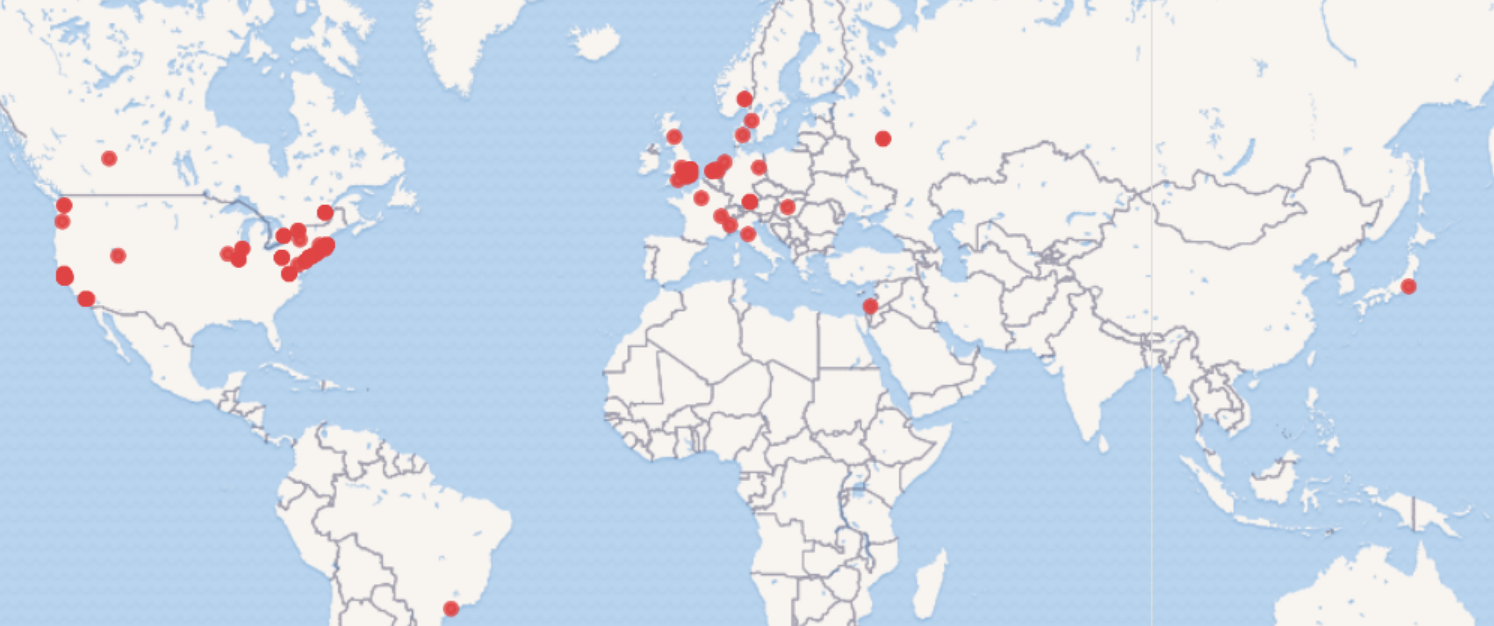
\includegraphics[width=1\textwidth]{./chapter/programming_language/Map_showing_educational_institutes_2017.png}
	\caption{Учебные заведения, в которых учились люди, создававшие языки программирования (2017).}
	\label{fig:universities_2017}
\end{figure}
\begin{figure}[h]
\centering
	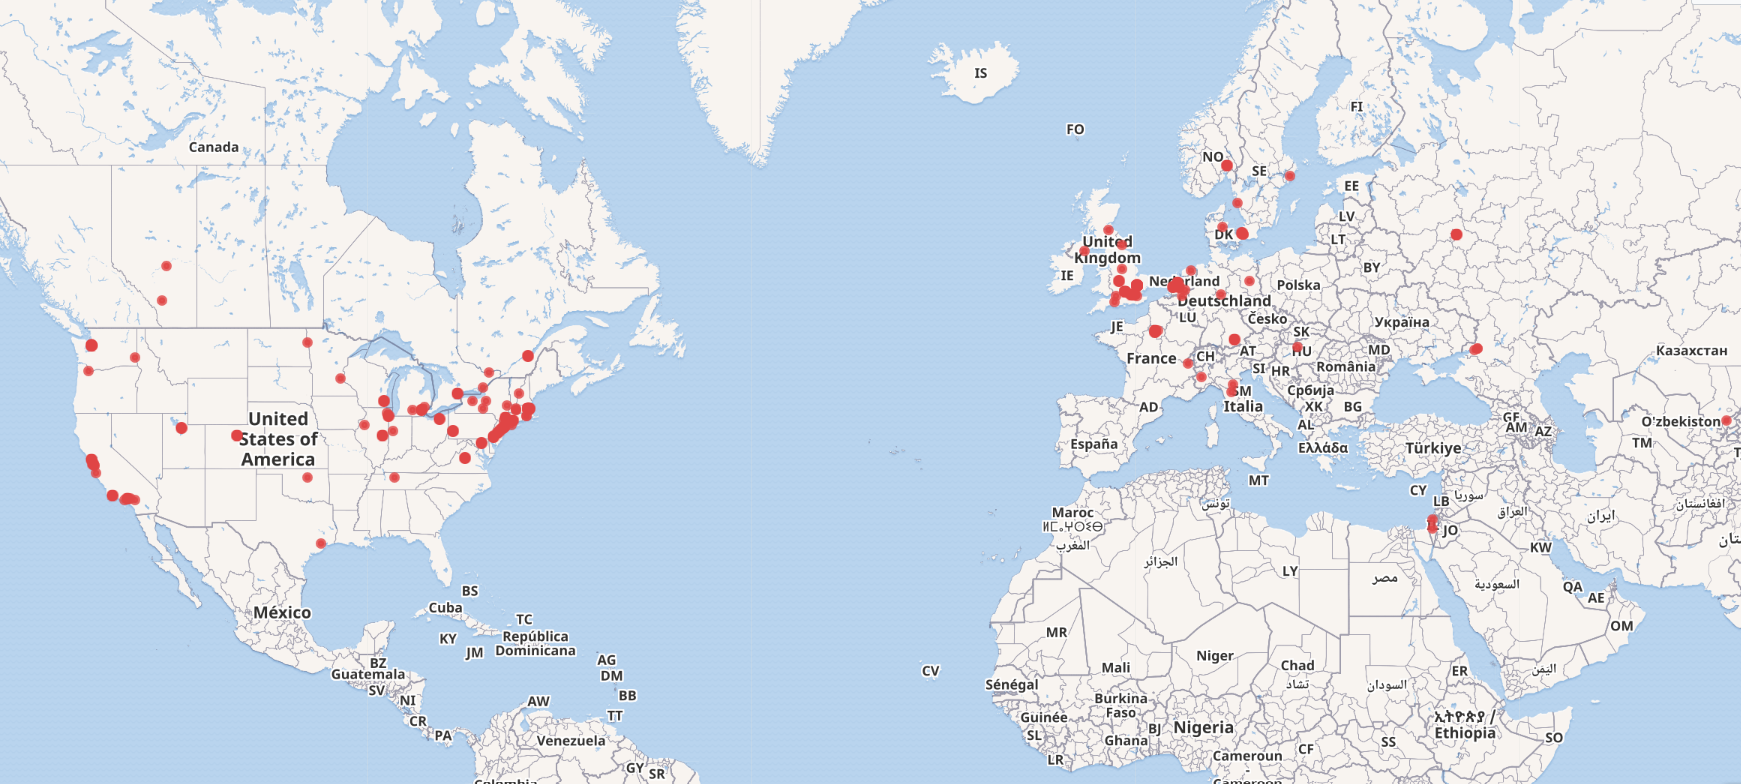
\includegraphics[width=1\textwidth]{./chapter/programming_language/Map_showing_educational_institutes_2020.png}
	\caption{Учебные заведения, в которых учились люди, создававшие языки программирования (2020).}
	\label{fig:universities_2020}
\end{figure}


По картам~\ref{fig:universities_2017} и~\ref{fig:universities_2020} видно, что большая часть людей, причастных к созданию языков программирования, учились в Европе или в США и динамика не сильно изменилась за 3 года.

Построим также пузырьковую-диаграмму (запрос~\ref{lst:developer_universities_bubble}) по самым популярным учебным заведениям, среди будущих создателей языков программирования. Видим на рисунке, что на первых местах оказались: Принстонский университет (8 студентов) и Стэнфордский университет (8). МГУ оказался в конце списка, в нем учился Энтони Ричард Хоар, разработавший ALGOL60, и Валентин Фёдорович Турчин, разработавший РЕФАЛ. МГУ попал в этот список, включающий 142 вуза мира.

\begin{lstlisting}[
	language=SPARQL,
	label=lst:developer_universities_bubble,
	caption={\href{https://w.wiki/kDb}{Университеты, у которых учились разработчики языков программирования}\protect\footnotemark},
	texcl
]
#2017-05
#defaultView:BubbleChart
SELECT ?educational_institution_label (count(*) as ?count)
WHERE
{
 ?item wdt:P31 wd:Q9143 # instances of programming language
 ; rdfs:label ?item_label. 
 FILTER (LANG(?item_label) = "en"). 
 
 ?item wdt:P178 ?developer. # developer
 ?developer rdfs:label ?developer_label. 
 FILTER (LANG(?developer_label) = "en"). 
 	
 ?developer wdt:P69 ?educational_institution. # educated at
 ?educational_institution rdfs:label ?educational_institution_label. 
 FILTER (LANG(?educational_institution_label) = "en").
 
 ?educational_institution wdt:P625 ?coord. # coordinate location
 
 SERVICE wikibase:label {
 bd:serviceParam wikibase:language "en".
 } 	
}
GROUP BY ?educational_institution_label
ORDER BY DESC(?count)
\end{lstlisting}

%%
% Профессии создателей языков программирования
%%
\section{Профессии создателей языков программирования}
Построим пузырьковую диаграмму (~\ref{lst:developer_profession}), отображающую какие профессии преобладают среди людей, разрабатывающих языки программирования.

Используются:
\begin{itemize}
\itemОбъект: programming language (Q9143).
\itemСвойство: instance of (P31).
\itemСвойство: developer (P178).
\itemСвойство: occupation (P106).
\end{itemize}

\begin{lstlisting}[
	language=SPARQL,
	label=lst:developer_profession,
	caption={\href{https://w.wiki/kDc}{Профессии создателей языков программирования}\protect\footnotemark},
	texcl
]
#2017-05
#defaultView:BubbleChart
SELECT ?occupation_label (count(*) as ?occupation)
WHERE
{
    ?item wdt:P31 wd:Q9143. # instances of programming language 
    ?item wdt:P178 ?developer. # developer
    ?developer wdt:P106 ?occupation. # occupation
    ?occupation rdfs:label ?occupation_label. 
    FILTER (LANG(?occupation_label) = "ru"). 
}
GROUP BY ?occupation_label 
ORDER BY DESC(?count)
\end{lstlisting}

\begin{marginfigure}
{
\setlength{\fboxsep}{0pt}%
\setlength{\fboxrule}{1pt}%
\fcolorbox{white}{white}{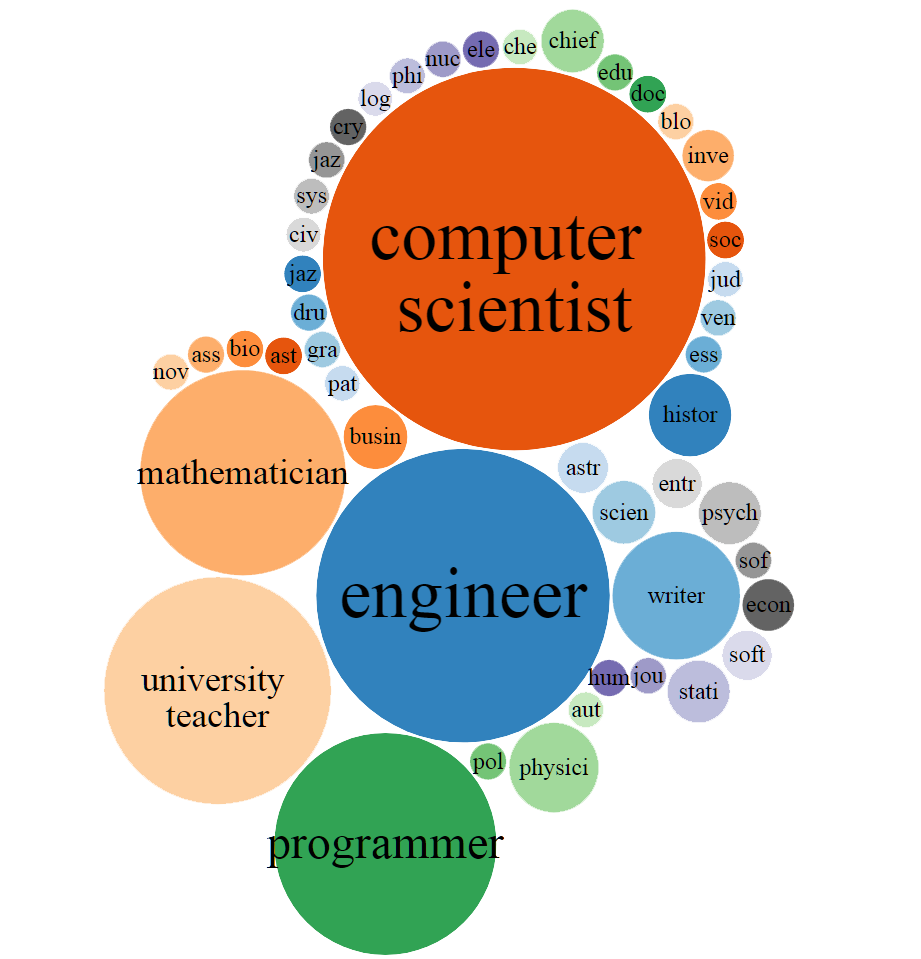
\includegraphics[width=\linewidth]{./chapter/programming_language/Bubble_chart_showing_the_quantity_of_professions_people_,creating_programming_languages,_have_2017.png}}%
}
  \caption{Профессии людей, которые разрабатывают языки программирования (2017).}%
  \label{fig:profession_2017}%
\end{marginfigure}
\begin{marginfigure}
{
\setlength{\fboxsep}{0pt}%
\setlength{\fboxrule}{1pt}%
\fcolorbox{white}{white}{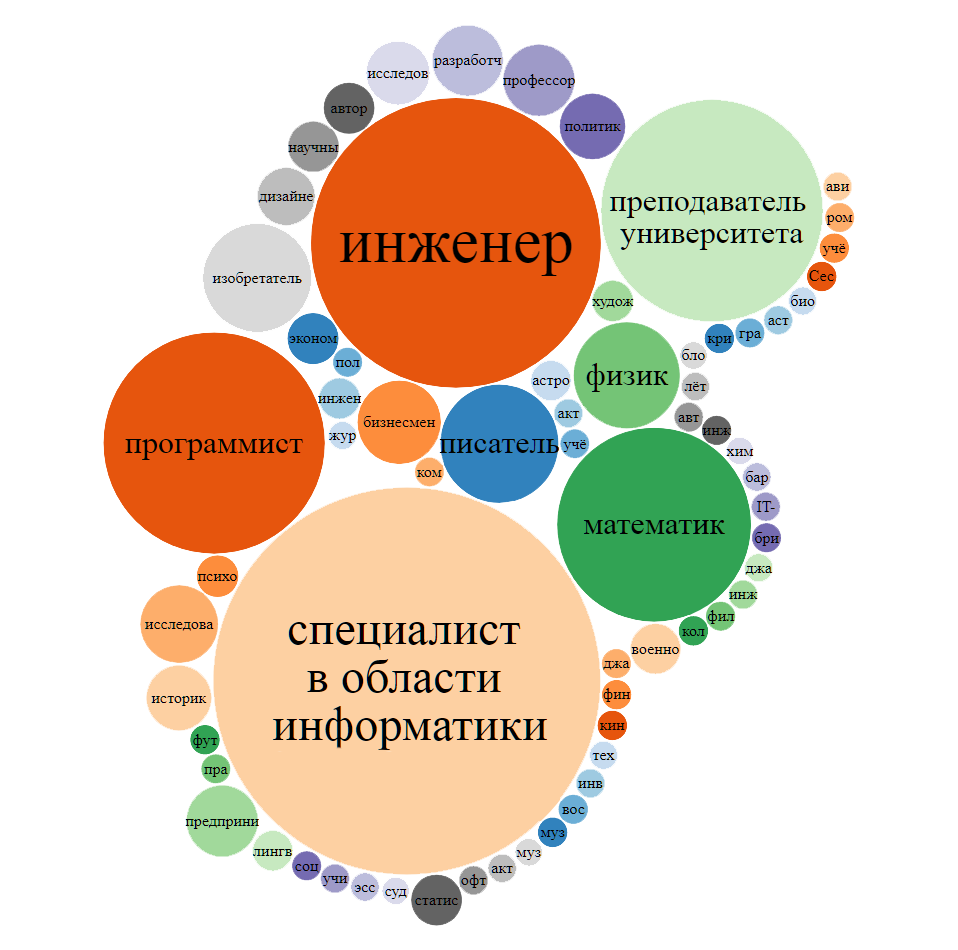
\includegraphics[width=\linewidth]{./chapter/programming_language/Bubble_chart_showing_the_quantity_of_professions_people,_creating_programming_languages_RU_2020.png}}%
}
  \caption{Профессии людей, которые разрабатывают языки программирования (2020).}%
  \label{fig:profession_2020}%
\end{marginfigure}
\footnotetext{Результатом запроса~\ref{lst:developer_profession} в 2017 году является 48 записей, к 2020 году их число увеличилось до 74.}

Результаты запросов можно выдеть на рисунках~\ref{fig:profession_2017} и~\ref{fig:profession_2020}.
Наиболее распространенными профессиями оказались: специалист в области компьютерных наук, инженер, учитель. Интересно заметить, что встречаются такие профессии как: джазовый музыкант, политик (Герберт Александер Саймон). На 2020 год среди разработчиков языков программирования оказалось больше всего специалистов в области компьютерных наук (172 человека), а также 96 инженеров, 57 учителей, 56 программистов и 43 математика.

%%
% Объектно-ориентированные языки программирования
%%
\section{Объектно-ориентированные языки программирования}
Вывести список всех объектно-ориентированных языков программирования.

Используются:
\begin{itemize}
\itemОбъект: object-oriented programming language (Q899523).
\itemСвойство: instance of (P31).
\end{itemize}

\begin{lstlisting}[
	language=SPARQL,
	label=lst:oopl,
	caption={\href{https://w.wiki/kDe}{Список объектно-ориентированных языков программирования}\protect\footnotemark},
	texcl
]
#2017-4
SELECT DISTINCT ?item ?item_label
WHERE
{
    ?item wdt:P31 wd:Q899523 # instances of object-oriented programming language
    ; rdfs:label ?item_label . 

    FILTER (LANG(?item_label) = "ru") . 
}
\end{lstlisting}

\footnotetext{Результатом SPARQL-запроса~\ref{lst:oopl} является список объектно-ориентированных языков программирования. На 2017 год список содержал 116 записей, к 2020 году число записей увеличилось на 2 и составляет 118 языков программирования.}

Таким образом 8\% языков программирования на 2020 год являются объектно-ориентированными.

%%
% Полнота викиданных
%%
\section{Полнота викиданных}
По данным Боровского исследовательского университета существует как минимум 26 языков программирования, которые поддерживают объектно-ориентированную парадигму. В статьях посвященных объектно-ориентированному программированию к этому списку добавляются ещё 4 и 3 языка программирования. 

\begin{lstlisting}[
	language=SPARQL,
	label=lst:fullness,
	caption={\href{https://w.wiki/kDf}{Смотрим на полноту викиданных}\protect\footnotemark},
	texcl
]
#2017-4
SELECT DISTINCT ?item ?item_label
WHERE
{
 ?item wdt:P31 wd:Q899523 # instances of object-oriented programming language
 ; rdfs:label ?item_label . 

 FILTER (LANG(?item_label) = "en")
}
\end{lstlisting}
\footnotetext{SPARQL-запрос~\ref{lst:fullness} вернул 119 результатов.}

Судить о полноте данных в трех приведенных выше источниках сложно, так как большое количество малоизвестных, устаревших и узконаправленных языков, которые не освещаются в авторитетных источниках. Из этого можно сделать вывод, Викиданные предоставляют достаточно полный список объектно-ориентированных языков программирования.

%%
% Заполнение объектов
%%
\section{Заполнение объектов}
Выведем список всех людей, которые связаны с разработкой языков программирования и у объектов которых заполнено поле "label"\  на английском языке:

\begin{lstlisting}[
	language=SPARQL,
	label=lst:filling,
	caption={\href{https://w.wiki/kDg}{Список разработчиков языков программирования с заполненным полем label}\protect\footnotemark},
	texcl
]
#2017-05
SELECT ?item_label ?item ?developer_label ?developer
WHERE
{
    ?item wdt:P31 wd:Q9143 # instances of programming language
    ; rdfs:label ?item_label. 
    FILTER (LANG(?item_label) = "ru"). 

    ?item wdt:P178 ?developer. # developer 
    ?developer wdt:P31 wd:Q5.  # instances of human
    ?developer rdfs:label ?developer_label. 
    FILTER (LANG(?developer_label) = "ru").  
}
\end{lstlisting}
\footnotetext{По результату запроса~\ref{lst:filling} в на 21 мая 2017 года было получено 133 записи, в 2020 году получено 223 записи.}
Выведем аналогичный список, но с заполненным полем "label"\  на русском языке. Таких записей 88. Заполним поля "label"\  и "description"\  на русском языке у этих объектов и выведем результат:

\begin{lstlisting}[
	language=SPARQL,
	label=lst:filling_label,
	caption={\href{https://w.wiki/kDj}{Список разработчиков языков программирования с заполненным полем label и description}\protect\footnotemark},
	texcl
]
#2017-05
SELECT ?item_label ?item ?developer_label ?developer
WHERE
{
    ?item wdt:P31 wd:Q9143 # instances of programming language
    ; rdfs:label ?item_label. 
    FILTER (LANG(?item_label) = "ru"). 

    ?item wdt:P178 ?developer. # developer 
    ?developer wdt:P31 wd:Q5.  # instances of human
    ?developer rdfs:label ?developer_label. 
    FILTER (LANG(?developer_label) = "ru").  
}
\end{lstlisting}
\footnotetext{В 2017 году запрос~\ref{lst:filling_label} вернул 133 значения, в 2020 году выполнение запроса дало 183 записи.}